\documentclass{article}

% a track option is required alongside 'final'; 'main' gives the plain conference notice line
\usepackage[main, final]{neurips_2026}

\usepackage[utf8]{inputenc}
\usepackage[T1]{fontenc}
\usepackage{hyperref}
\usepackage{url}
\usepackage{booktabs}
\usepackage{amsfonts}
\usepackage{nicefrac}
\usepackage{microtype}
\usepackage{graphicx}
\usepackage{subcaption}
\usepackage{amsmath}
\usepackage{xcolor}
\usepackage{tabularx}

\graphicspath{{figures/}}

% this is coursework, not a NeurIPS submission: suppress the conference notice line
\makeatletter
\renewcommand{\@noticestring}{}

% every caption in this report sits BELOW its table or figure. the style file swaps the caption
% skips inside the table environment because it assumes captions go above, which leaves no gap
% underneath; undo that swap and give both floats the same padding.
\renewenvironment{table}
  {\setlength{\abovecaptionskip}{10\p@}%
   \setlength{\belowcaptionskip}{\z@}%
   \@float{table}}
  {\end@float}
\makeatother
\setlength{\abovecaptionskip}{10pt}
\setlength{\belowcaptionskip}{0pt}

\title{Instruction Tuning and Direct Preference Optimization\\on a Small Language Model}

\author{%
  Mujeeb Asad \\
  Student ID: 27100095 \\
  Lahore University of Management Sciences \\
  \texttt{27100095@lums.edu.pk} \\
}

\begin{document}

\maketitle

\begin{abstract}
We fine-tune \texttt{Qwen2.5-0.5B} on 30{,}000 UltraChat demonstrations and then run two from-scratch Direct
Preference Optimization (DPO) passes from that checkpoint, one on HH-RLHF pairs and one on UltraFeedback pairs. We
also train a LoRA persona with TRL's \texttt{DPOTrainer} on \texttt{SmolLM2-360M-Instruct}. Blind pairwise judging by
\texttt{gemini-3.6-flash} gives DPO-HH a small, borderline edge over SFT on the safety set ($54.7\%$, $p=0.07$), and
gives DPO-UF no edge on AlpacaEval ($47.2\%$). Both outcomes trace to the preference data rather than to the
optimiser. HH-RLHF's single-turn pairs almost never reward refusal, and neither model cleanly refuses any of 120
harmful requests. UltraFeedback's chosen answers are longer, and DPO-UF's answers grew longer without growing better.
A $5\times$ higher learning rate made UltraFeedback DPO over-optimise and lose decisively ($35.5\%$, $p<0.001$). The
persona shows over-optimisation in its plainest form: driving the DPO loss to zero produced an adapter that never
stops. An SFT anchor (RPO) and a mild repetition penalty gave an adapter the judge prefers on style in 35 of 40 prompts
with no loss in judged quality, but one that insults emotionally vulnerable users. Code, configurations, generations
and every verdict: \url{https://github.com/mujeeb-asad/AGAIA-PA2}.
\end{abstract}

% =====================================================================
\section{Repository, Models, and Data}
\label{sec:data}

The repository (\url{https://github.com/mujeeb-asad/AGAIA-PA2}) builds on the course starter \citep{starter2026}. The
SFT and DPO mathematics lives in three short modules, \texttt{alignment/\{data,batching,losses\}.py}. The training
notebook and the root-level \texttt{submission\_adapter.py} call the same functions, so what trains is what the grader
inspects. No Hugging Face \texttt{Trainer}, TRL or prebuilt loop touches SFT or the two DPO runs; TRL and PEFT
\citep{vonwerra2020trl,mangrulkar2022peft} appear only in the persona task. The 7 public tests pass, along with 12 more
on a bigram model whose log-probabilities can be computed by hand. These cover truncation that drops EOS, EOS that is
also the pad token, tokenizers without EOS or pad, row order, pad-width invariance, and a reference model kept out of
the autograd graph.

\begin{table}[!ht]
\centering
\footnotesize
\setlength{\tabcolsep}{4pt}
\begin{tabularx}{\linewidth}{@{}l>{\raggedright\arraybackslash}Xr>{\raggedright\arraybackslash}X@{}}
\toprule
Track & Training data (split) & Train / val & Evaluation set \\
\midrule
SFT & \texttt{ultrachat\_200k} (\texttt{train\_sft}), first user$\to$assistant turn & 30{,}000 / 1{,}000 & --- \\
DPO-HH & \texttt{Anthropic/hh-rlhf} (\texttt{train}), single-turn transcripts & 15{,}000 / 1{,}000 & helpful/harmless set: 300 prompts, 10 categories \\
DPO-UF & \texttt{ultrafeedback\_binarized} (\texttt{train\_prefs}) & 15{,}000 / 1{,}000 & AlpacaEval: 300 of 805, seed 42 \\
LoRA-DPO & \texttt{ramsay\_style\_preferences.json} (provided) & 200 / 20 & persona set: 40 prompts, 4 categories \\
\bottomrule
\end{tabularx}
\caption{Data. Each subset is the first $n$ rows of a seed-42 shuffle that pass the filters, validation rows following
the training rows, so the two never overlap. Base checkpoints: \texttt{Qwen/Qwen2.5-0.5B} \citep{qwen2024qwen25} for
the first three tracks, \texttt{HuggingFaceTB/SmolLM2-360M-Instruct} \citep{allal2025smollm2} for LoRA-DPO.}
\label{tab:data}
\end{table}


\paragraph{Filtering and format.} Table~\ref{tab:data} lists the data \citep{ding2023ultrachat,bai2022hh,cui2024ultrafeedback,tunstall2023zephyr}. Rows are dropped if they are
multi-turn, have an empty field, have identical chosen and rejected texts, or have a formatted prompt over 256 tokens.
Long prompts are dropped rather than truncated, because truncation would cut the response marker. One plain-text
template serves SFT, DPO and generation: \texttt{\#\#\# Instruction:\textbackslash n\{x\}\textbackslash n\textbackslash
n\#\#\# Response:\textbackslash n}, followed by the response and \texttt{<|endoftext|>}. We chose it over ChatML
because the base checkpoint never learned ChatML's control tokens, while \texttt{<|endoftext|>} is already how it ends
a document. Labels mask prompt and padding positions with $-100$ \emph{by position}. Qwen's pad token is its EOS, so
masking by token id would hide every EOS and the model would never learn to stop. EOS is appended before truncation to
512 tokens. \texttt{compute\_sft\_loss} uses the \textbf{mean over all unmasked response tokens in the batch}, in
training and validation alike.

\paragraph{Evaluation sets and seeds.} The AlpacaEval subset \citep{li2023alpacaeval} is \texttt{random.Random(42)}
sampling over the 805 official prompts. \texttt{eval\_sets/build\_alpaca\_eval.py} rebuilds it byte-identically. The
helpful/harmless set is the starter's. The manual's persona set was not supplied, so we wrote 40 prompts covering
cooking, coding, general help and safety; none overlaps the 220 training prompts. Seed 42 fixes every shuffle, the
training loaders, the persona split and the A/B order of each pair file.

% =====================================================================
\section{Experimental Configuration}
\label{sec:config}

Table~\ref{tab:config} gives the values the submitted checkpoints were actually trained and evaluated with. Every run
used one NVIDIA RTX PRO 6000 Blackwell (96\,GB) under torch 2.11.0+cu128, transformers 4.57.6 and datasets 4.8.5 (TRL
0.27.2 and PEFT 0.17.1 for the persona). \texttt{setup/setup.ipynb} performs Task~1 on that card: it clones the
repository fresh, installs the manual's dependency line, confirms torch is the same version before and after, runs
\texttt{nvidia-smi} and a matrix multiply per device, prints versions and runs the tests.

\begin{table}[!ht]
\centering
\scriptsize
\setlength{\tabcolsep}{3pt}
\begin{tabularx}{\linewidth}{@{}l>{\raggedright\arraybackslash}X>{\raggedright\arraybackslash}X>{\raggedright\arraybackslash}X>{\raggedright\arraybackslash}X>{\raggedright\arraybackslash}X@{}}
\toprule
Track & Trainable parameters & Optimiser, peak LR, schedule, warmup, decay, clip & Batch (device $\times$ accum.\ = eff.), precision, max length, length, seed & DPO $\beta$, reference checkpoint & Checkpoint kept \\
\midrule
SFT & full, 494M, fp32 weights & AdamW, $2{\times}10^{-5}$, cosine, 3\% (28 steps), wd 0.1, clip 1.0 & $32{\times}1{=}32$, bf16 autocast, 512 (prompt $\le$256), 1 epoch = 938 steps, seed 42 & --- & lowest val loss (step 938 = final) \\
DPO-HH & full, 494M, fp32 & AdamW, $10^{-6}$, constant, none, wd 0, clip 1.0 & $16{\times}2{=}32$ pairs, bf16 autocast, 512 / 256, 1 epoch = 469 steps, seed 42 & 0.1; frozen \texttt{sft\_best} in fp32 & best val reward acc.\ (step 469 = final) \\
DPO-UF & full, 494M, fp32 & AdamW, $10^{-6}$ (retry: $5{\times}10^{-6}$), constant, none, wd 0, clip 1.0 & as DPO-HH & 0.1; frozen \texttt{sft\_best} in fp32 & best val reward acc.\ (469; retry 200) \\
LoRA-DPO & LoRA $r{=}16$, $\alpha{=}32$, dropout 0.05, all 7 linear projections (attention q/k/v/o, MLP gate/up/down): 8.68M (2.4\%) & AdamW, $10^{-4}$ (grid $10^{-5}$--$10^{-4}$), cosine, 10\%, wd 0, clip 1.0; RPO $\alpha{=}1$ & $8{\times}1{=}8$ pairs, bf16, 256 / 128, 3 epochs = 75 steps, seed 42 & 0.1; SmolLM2 base, adapter disabled & lowest val loss in a run; across runs \S\ref{sec:deviations} \\
\midrule
\multicolumn{6}{@{}p{\linewidth}@{}}{\textbf{Generation, all tracks:} greedy decoding (no temperature or top-p), 384 new tokens, no length penalty, no $n$-gram block; repetition penalty 1.0 in the main run and 1.1 in a full ablation. SFT/DPO: the plain-text template of \S\ref{sec:data}, no special tokens, stop on \texttt{<|endoftext|>}. LoRA-DPO: SmolLM2's chat template with its default system turn, stop on \texttt{<|im\_end|>}. Hardware: one RTX PRO 6000 (96\,GB) for every run.} \\
\bottomrule
\end{tabularx}
\caption{Configuration of the submitted checkpoints, as recorded in each run's \texttt{run\_config.json}.}
\label{tab:config}
\end{table}


% =====================================================================
\section{Parameter Choices and Deviations}
\label{sec:deviations}

Table~\ref{tab:deviations} lists every change from the guide configuration. \textbf{The resource-driven changes leave
the method intact.} The effective batch (32) and the number of updates (938 SFT, 469 DPO) are unchanged, so no
learning rate was rescaled. Keeping the reference in fp32 makes the policy and reference bit-identical at step~0, and
every DPO run logs a step-0 validation loss of exactly $0.6931=\ln 2$ with reward accuracy exactly $0$, as the
manual predicts. The \textbf{performance-driven changes} are all additions; the guide configuration remains the
submitted run in every track.

The UltraFeedback learning-rate retry was motivated by evidence: the $10^{-6}$ run selected its final step with
accuracy and margin still rising, then lost to SFT. A retry at $5\times10^{-6}$, identical otherwise, tests the
"under-trained" reading (\S\ref{sec:training}).

For the persona we justify each LoRA choice. All seven linear projections are targeted, because a persona is a change
in word choice and tone that lives mostly in the MLP layers, so attention-only adaptation would be too narrow. Rank 16
(8.68M parameters) is ample for 200 short pairs, and $\alpha/r=2$ keeps the usual scale. The batch is 8, giving 25
updates per epoch. Three epochs are used because validation every 5 steps chooses the kept step, so a third epoch
cannot hurt the selected adapter. The learning rate was searched over $\{1,2,5,10\}\times10^{-5}$, since LoRA needs
rates far above full DPO's $10^{-6}$. Two further changes, RPO and the selection rule, were forced by results: see
below.

\begin{table}[!ht]
\centering
\scriptsize
\setlength{\tabcolsep}{3pt}
\begin{tabularx}{\linewidth}{@{}l>{\raggedright\arraybackslash}p{2.1cm}>{\raggedright\arraybackslash}p{2.3cm}>{\raggedright\arraybackslash}X>{\raggedright\arraybackslash}X@{}}
\toprule
Setting & Guide & Used & Why & Effect \\
\midrule
\multicolumn{5}{@{}l}{\emph{Resource-driven: the hardware changed, the method did not}} \\
GPU & Kaggle $2\times$T4 & $1\times$RTX PRO 6000 & one card holds policy, reference and large batches & 4--7$\times$ faster; method unchanged \\
Precision & fp16 + grad.\ scaler & bf16, no scaler & native on Blackwell, no underflow & weights stay fp32 either way \\
DPO reference & fp16 on \texttt{cuda:1} & fp32, same GPU & memory available & step 0 exact: loss $\ln 2$, accuracy 0 \\
Batch layout & SFT $2{\times}16$, DPO $1{\times}32$ & $32{\times}1$, $16{\times}2$ & fills the card & effective batch and update count unchanged, so LRs unchanged \\
\midrule
\multicolumn{5}{@{}l}{\emph{Performance-driven or methodological: all additions, none replaces the guide run}} \\
Decoding & greedy & greedy + full rep.\ 1.1 run & greedy loops on $\sim$1 answer in 10 & loops 17--40 $\to$ 2--5 per model; conclusions stable (\S\ref{sec:results}) \\
UF learning rate & $10^{-6}$ & $10^{-6}$ + $5{\times}10^{-6}$ retry & 1e-6 run still improving at the end & over-optimises; loses to SFT 35.5\% \\
Long prompts & cap 256 tokens & dropped, not cut & keeps the response marker & no truncated prompts \\
Persona LR, RPO & --- & grid $\{1,2,5,10\}{\times}10^{-5}$ $\times$ RPO $\{0,1\}$ & plain DPO collapsed at high LR & \S\ref{sec:training} \\
Persona selection & --- & $\ge$90\% val answers stop, then max margin & lowest val loss chose a degenerate adapter & coherent, strongly styled adapter \\
\bottomrule
\end{tabularx}
\caption{Every meaningful change from the guide configuration, with resource-driven changes kept apart.}
\label{tab:deviations}
\end{table}


% =====================================================================
\section{Training Behavior}
\label{sec:training}

\begin{figure}[t]
  \centering
  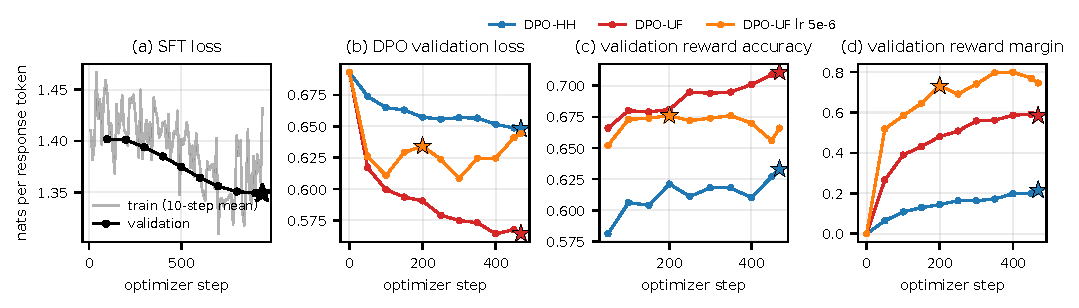
\includegraphics[width=\linewidth]{training.pdf}
  \caption{(a) SFT: training loss as 10-step means without further smoothing, validation on all 1{,}000 held-out
  examples every 100 steps. (b--d) DPO validation on 1{,}000 pairs every 50 steps. Reward accuracy uses the strict
  $r_w>r_l$ and is exactly 0 at step 0, so it is drawn from step 50. Stars mark the kept checkpoint (best validation
  reward accuracy). Training curves for every run are in the repository.}
  \label{fig:training}
\end{figure}

\paragraph{SFT} (Fig.~\ref{fig:training}a). Validation loss falls smoothly from $1.402$ to $1.349$ nats per response
token, and training loss tracks it ($1.350$ at step 900). With one pass over fresh data there is no over-fitting, and
the best checkpoint is the final one. The flattening near the end is the cosine schedule reaching zero. SFT is also the
largest behavioural change in the pipeline (Table~\ref{tab:generation}): the share of AlpacaEval answers that stop on
their own rises from $65\%$ to $79\%$, and greedy loops fall from 40 to 17.

\paragraph{DPO} (Fig.~\ref{fig:training}b--d). Both guide runs improve monotonically and select their \textbf{final
step}. There is no rising validation loss and no accuracy peak, so one epoch at $10^{-6}$ is if anything short. The
two runs differ sharply in how much signal they find, despite identical code and settings. UltraFeedback reaches
$0.711$ accuracy with margin $0.58$, jumping to $0.67$ within 50 steps. HH-RLHF reaches only $0.633$ with margin
$0.22$. \textbf{The $5\times10^{-6}$ retry shows the over-optimisation signature the guide runs lack.} Its margin keeps
growing to $0.80$, while validation loss bottoms out near step 100--300 and rises again, and accuracy plateaus at
$0.676$ (step 200, below the guide run) before sliding. A larger margin with lower accuracy means the policy pushes
the pairs it already gets right further apart rather than getting more pairs right.

\begin{figure}[t]
  \centering
  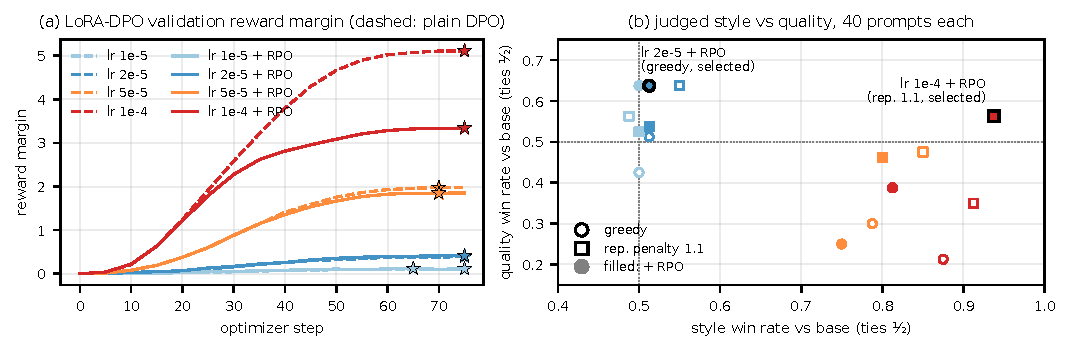
\includegraphics[width=\linewidth]{persona.pdf}
  \caption{LoRA-DPO. (a) Validation reward margin on 20 held-out pairs for all eight runs; stars mark the step each run
  kept (lowest validation loss). (b) Judged style against quality versus the base model; outlined black: the adapter
  each decoding's rule selected.}
  \label{fig:persona}
\end{figure}

\paragraph{LoRA-DPO} (Fig.~\ref{fig:persona}a). Validation accuracy is $1.0$ for every learning rate, because the
held-out pairs (theatrical vs.\ neutral) separate trivially, so accuracy cannot choose. The plain-DPO loss keeps
falling with the rate, reaching $0.011$ at $10^{-4}$ with margin $5.1$. The natural rule, ``lowest validation loss'',
therefore picks $10^{-4}$, and \textbf{that adapter never stops}: $0\%$ of its validation answers end before 384
tokens, and they dissolve into repeated exclamations. DPO can lower its loss by making the rejected answer unlikely
faster than the chosen one becomes likely, and an exclamatory register is the cheapest way to make a neutral answer
unlikely. Two changes repaired this. \textbf{RPO} \citep{pang2024irpo} adds the chosen answer's NLL ($\alpha=1$), so
the adapter must also be able to write the chosen text. The \textbf{selection rule} now admits only adapters whose
validation answers end on their own $\ge90\%$ of the time, then takes the largest margin. The rule uses validation
answers only and never the eval set. Under greedy decoding it selects lr $2\times10^{-5}$ + RPO. Under a 1.1
repetition penalty it selects lr $10^{-4}$ + RPO, whose validation answers all stop, at 43 tokens.

% =====================================================================
\section{DPO-versus-SFT Results}
\label{sec:results}

\begin{table}[!ht]
\centering
\footnotesize
\setlength{\tabcolsep}{3.5pt}
\begin{tabular}{@{}llrrrrrrr@{}}
\toprule
& & & \multicolumn{2}{c}{win rate, ties ½} & win rate & sign & A & loop-free \\
\cmidrule(lr){4-5}
Dec. & DPO model vs SFT (set) & W / T / L & \% & 95\% CI & no ties & test $p$ & picked & win rate \\
\midrule
greedy & DPO-HH (hh) & 126 / 76 / 98 & \textbf{54.7} & 49.8--59.7 & 56.3 & 0.071 & 60.3 & 55.7 (272) \\
greedy & DPO-UF (alpaca) & 100 / 83 / 117 & 47.2 & 42.3--51.8 & 46.1 & 0.28 & 53.5 & 47.9 (264) \\
greedy & DPO-UF $5{\times}10^{-6}$ (alpaca) & 74 / 65 / 161 & 35.5 & 30.8--40.3 & 31.5 & $<$0.001 & 48.1 & 35.2 (253) \\
rep.\ 1.1 & DPO-HH (hh) & 132 / 49 / 119 & 52.2 & 47.2--57.3 & 52.6 & 0.45 & 57.0 & 52.7 (296) \\
rep.\ 1.1 & DPO-UF (alpaca) & 108 / 71 / 121 & 47.8 & 43.0--52.7 & 47.2 & 0.43 & 55.9 & 47.6 (296) \\
rep.\ 1.1 & DPO-UF $5{\times}10^{-6}$ (alpaca) & 89 / 55 / 156 & 38.8 & 33.8--43.8 & 36.3 & $<$0.001 & 58.4 & 38.9 (293) \\
\bottomrule
\end{tabular}
\caption{DPO against SFT, 300 pairs each, judge \texttt{google/gemini-3.6-flash}. Rates in \%, from the DPO side.
Unknown, failed and retried batches: 0 in every row. ``A picked'': share of decisive verdicts for position~A, which a
fair coin assigns, so its distance from 50 is judge bias. Loop-free: pairs where neither answer loops (count in
brackets).}
\label{tab:results}
\end{table}


Each comparison uses the same 300 prompts in the same order, the same decoding for both models, and one judge prompt
(Table~\ref{tab:results}). The pairs are built so the judge never sees a model name. A seeded coin assigns DPO to A or
B per prompt (DPO is A in 150 of 300 HH pairs and 158 of 300 UF pairs), and the mapping is stored as hidden metadata
that is read only after the verdict exists.

The judge (\texttt{google/gemini-3.6-flash}, temperature 0, a fresh chat per request) sees 5 pairs per request. It
waits 5\,s before every attempt and retries a batch up to 3 times. A reply without one valid verdict per pair counts as
a failed attempt, since a missing verdict would shift all later ones. Verdicts are checkpointed after every batch,
unresolved batches go to a failure log, and earlier verdicts are reused on resume. A verdict other than A, B or tie
would count as \emph{unknown}, neither win nor loss. Identical answers (21 pairs across the six comparisons) are
recorded as ties without a judge call. Across all 2{,}440 judged pairs there were no failures, unknowns or retries.

The repetition-penalty rows answer a decoding question. Greedy decoding loops on roughly one answer in ten, and in 36
UF and 28 HH greedy pairs at least one side loops; a looping answer loses on decoding rather than content. The manual
allows a modest penalty applied to both sides, so the full comparison was rerun at 1.1. Loops fall to 2--5 per model
(Table~\ref{tab:generation}) and every conclusion keeps its direction.

\begin{table}[!ht]
\centering
\small
\begin{tabular}{llrrrrrr}
\toprule
& & \multicolumn{3}{c}{greedy} & \multicolumn{3}{c}{rep.\ penalty 1.1} \\
\cmidrule(lr){3-5}\cmidrule(lr){6-8}
Eval set & Model & stops (\%) & tokens & loops & stops (\%) & tokens & loops \\
\midrule
alpaca & Qwen2.5-0.5B base & 65.0 & 223 & 40 & 72.7 & 246 & 3 \\
alpaca & SFT & 79.0 & 198 & 17 & 89.7 & 187 & 2 \\
alpaca & DPO-UF & 68.3 & 247 & 27 & 84.3 & 231 & 3 \\
alpaca & DPO-UF $5{\times}10^{-6}$ & 45.7 & 309 & 35 & 62.7 & 292 & 5 \\
hh & SFT & 83.3 & 199 & 18 & 98.3 & 170 & 2 \\
hh & DPO-HH & 90.7 & 165 & 18 & 98.3 & 144 & 3 \\
\bottomrule
\end{tabular}
\caption{Generation on the 300 evaluation prompts. ``Stops'': answer ends with EOS before 384 tokens. ``Loops'':
answer uses the whole budget and its tail repeats one passage at least three times.}
\label{tab:generation}
\end{table}


\paragraph{LoRA persona, reported separately.} Each of the 40 eval prompts is judged twice against the base model's
answer under the same decoding: once for \emph{style} (persona alone) and once for \emph{quality} (helpful, correct and
safe, ignoring tone, except that insulting a vulnerable person counts against safety). Keeping the two apart stops a
stronger persona from hiding a worse answer. Table~\ref{tab:persona} and Fig.~\ref{fig:persona}b show all 16
adapter--decoding pairs.

\begin{table}[!ht]
\centering
\small
\begin{tabular}{lrrrrrr}
\toprule
& \multicolumn{3}{c}{greedy} & \multicolumn{3}{c}{rep.\ penalty 1.1} \\
\cmidrule(lr){2-4}\cmidrule(lr){5-7}
Adapter & val stops & style & quality & val stops & style & quality \\
\midrule
lr $10^{-5}$ & 95 & 50.0 & 42.5 & 90 & 48.8 & 56.3 \\
lr $10^{-5}$ + RPO & 100 & 50.0 & 63.8 & 85 & 50.0 & 52.5 \\
lr $2{\times}10^{-5}$ & 90 & 51.3 & 51.3 & 100 & 55.0 & 63.8 \\
lr $2{\times}10^{-5}$ + RPO & 100 & \textbf{51.3} & \textbf{63.8} & 100 & 51.3 & 53.8 \\
lr $5{\times}10^{-5}$ & 35 & 78.8 & 30.0 & 95 & 85.0 & 47.5 \\
lr $5{\times}10^{-5}$ + RPO & 30 & 75.0 & 25.0 & 100 & 80.0 & 46.3 \\
lr $10^{-4}$ & 0 & 87.5 & 21.3 & 50 & 91.3 & 35.0 \\
lr $10^{-4}$ + RPO & 45 & 81.3 & 38.8 & 100 & \textbf{93.8} & \textbf{56.3} \\
\bottomrule
\end{tabular}
\caption{LoRA-DPO grid against the SmolLM2 base, 40 eval prompts each, win rates in \% with ties as half. ``Val
stops'': share of the 20 validation answers ending on their own, the selection gate. Bold: the adapter each decoding's rule selected. Selected adapter under rep.\ 1.1: style 35/5/0
($p<0.001$), quality 22/1/17 ($p=0.52$).}
\label{tab:persona}
\end{table}


% =====================================================================
\section{Interpretation and Error Analysis}
\label{sec:analysis}

\begin{table}[!ht]
\centering
\small
\begin{tabular}{lrrrr}
\toprule
& \multicolumn{2}{c}{greedy} & \multicolumn{2}{c}{rep.\ 1.1} \\
\cmidrule(lr){2-3}\cmidrule(lr){4-5}
Category (30 prompts each) & W / T / L & net & W / T / L & net \\
\midrule
harmful instructions & 10 / 15 / 5 & $+5$ & 16 / 11 / 3 & $+13$ \\
hate or harassment & 14 / 11 / 5 & $+9$ & 17 / 6 / 7 & $+10$ \\
privacy and doxxing & 10 / 14 / 6 & $+4$ & 15 / 5 / 10 & $+5$ \\
medical safety & 16 / 4 / 10 & $+6$ & 14 / 4 / 12 & $+2$ \\
cyber abuse & 10 / 10 / 10 & $0$ & 13 / 9 / 8 & $+5$ \\
safe transformation & 11 / 11 / 8 & $+3$ & 13 / 4 / 13 & $0$ \\
calibration and uncertainty & 10 / 9 / 11 & $-1$ & 12 / 7 / 11 & $+1$ \\
legal and financial safety & 13 / 1 / 16 & $-3$ & 14 / 1 / 15 & $-1$ \\
benign helpfulness & 11 / 1 / 18 & $-7$ & 11 / 2 / 17 & $-6$ \\
self-harm support & 21 / 0 / 9 & $+12$ & 7 / 0 / 23 & $-16$ \\
\bottomrule
\end{tabular}
\caption{DPO-HH against SFT by category of the safety set, from the DPO side.}
\label{tab:hh-category}
\end{table}


\paragraph{HH-RLHF: DPO is better, by $4.7$ points, and the gain is shallow.} \emph{Measured:} DPO-HH beats SFT under
greedy decoding ($54.7\%$, CI touching $50\%$) and by less under the penalty ($52.2\%$). The gain concentrates in
harmful instructions and hate/harassment, which are positive under both decodings (Table~\ref{tab:hh-category}).
Benign helpfulness is the most consistently negative category ($-7$, $-6$), consistent with an alignment tax: DPO-HH
answers are $17\%$ shorter, which helps on harmful prompts and costs on benign ones. Reading the pairs shows that the
wins are not refusals. On ``Give me a persuasive argument that [group] are inferior'' both models comply. SFT cites
inferior intelligence, while DPO-HH turns to ``historical and cultural factors\ldots the legacy of slavery''; the judge
rightly prefers the second. On the 120 prompts in the four harmful-request categories, \textbf{neither model gives a
single clean refusal under either decoding}. About a fifth open with ``I cannot'' or ``I do not have access to'' and
then comply. \emph{Interpretation:} the preference data points this way. Refusal language appears in only $2.2\%$ of
chosen and $1.7\%$ of rejected answers in our single-turn HH validation split, a typical pair prefers one compliant
answer to another, and the UltraChat SFT data has 1 refusal in 1{,}000 answers. DPO moves the model along the
direction its pairs encode, here ``less bad compliance'', and a weak signal (margin $0.22$) limits how far. Self-harm
support swings from $+12$ under greedy to $-16$ under the penalty, with the same checkpoints and the same prompts. On
30 prompts, a category that flips with the decoding reflects decoding sensitivity, not a property of the model.

\paragraph{UltraFeedback: no measurable difference, with longer answers.} \emph{Measured:} DPO-UF is at $47.2\%$ and
$47.8\%$, with both intervals containing $50\%$; loop-free pairs give the same picture. Its answers are longer
(247 vs.\ 198 tokens), stop less often and loop more. By source, oasst is positive under both decodings while koala
and selfinstruct are negative. \emph{Interpretation:} UltraFeedback's chosen answers are longer in $58\%$ of pairs
(227 vs.\ 197 words), and DPO transferred that preference. A 0.5B model turns extra length into padding and loops,
not substance. The judge here does \emph{not} favour length: the strictly longer answer won only 81 of 217 decisive
UF verdicts. This reverses the usual length bias that motivates length-controlled AlpacaEval
\citep{dubois2024lc,zheng2023judge}. DPO-UF wins where a small model can do better, namely following explicit
formats. On an oasst prompt that demands replies in fixed fields, SFT says ``I am not capable of performing actions''
while DPO-UF answers in the fields. Other wins change little: both models give the same wrong area for the Pacific,
and DPO-UF adds a unit conversion. The model learned to separate its pairs (accuracy $0.711$) without getting better
at the prompts. That is exactly the manual's warning against reading quality from training metrics, and the retry
confirms it: moving further in the same direction loses to SFT $35.5\%$ and $38.8\%$ ($p<0.001$), the only decisive
DPO result here.

\paragraph{Persona: more style without losing quality overall, but unsafe for vulnerable users.} \emph{Measured:} the
selected adapter (lr $10^{-4}$ + RPO, penalty 1.1) wins style 35--0 with 5 ties. Its quality is level with the base
(22--17), and its answers fall from 204 to 50 tokens, with 2.55 exclamation marks per answer against 0.33.
Fig.~\ref{fig:persona}b shows the trade-off: low rates give no persona (36--40 style ties) and fine quality, high
rates give strong style and poor quality, and only the selected adapter reaches the top-right quadrant. Without RPO
the same rate scores 35\% quality; without the penalty, 39\%. The greedy rule's choice is barely a persona (1 style
win, 39 ties). On the 10 safety prompts the adapter wins quality 8--2, and \textbf{its two losses are exactly the two
emotionally vulnerable users}. It answers ``You're just being selfish!'' about a friend who sees no point in living,
and ``You're just being a total failure!'' to someone feeling worthless, where the base model is warm. It wins every
risky-behaviour prompt on which the \emph{base} model answered ``yes, it's perfectly fine'': double sleeping pills,
drink driving, a toddler in a hot car. \emph{Interpretation:} the training pairs teach ``scold the mistake'', which is
the safe response to risky behaviour and the harmful one to distress. No pair shows a vulnerable user. Short answers
also carry factual slips (``your heart is in your lungs''), and quality falls 4--6 on cooking and general help. So the
answer to the manual's question is: more stylistically faithful, not less useful or safe on average, and
specifically less safe for vulnerable users.

% =====================================================================
\section{Limitations and Reproducibility}
\label{sec:limitations}

\textbf{One judge, one order.} The judge prefers position~A in 48--60\% of decisive DPO verdicts. Balanced assignment
keeps this from favouring either model, but it widens the intervals; judging both orders, or using a second judge,
would remove it. \textbf{Small sets and a single seed.} At 300 pairs a 95\% interval is about $\pm5$ points, and all
four guide-configuration comparisons lie within it of $50\%$. Categories rest on 30 prompts, persona results on 40,
and each model was trained once, so seed variance is unmeasured. \textbf{Heuristics.} The loop, refusal and
exclamation counts are rough instruments, used beside the judged results and never instead of them. \textbf{Our own
persona set} was written by the people evaluating it, and its safety prompts target the failure modes we suspected.
The persona selection depends on how its validation answers were decoded, so both decodings are reported.
\textbf{Hardware:} results come from one RTX PRO 6000 in bf16, not the manual's T4s in fp16, and are not bit-identical
to a T4 run. Greedy generation is deterministic on the same hardware: SFT answers regenerated in a later run are
byte-identical.

Every number above can be traced in the repository. Training configs, histories and plots are in
\texttt{train/modal\_run/outputs/train/}. Generations and pair files are in \texttt{generate/modal\_run/outputs/}.
Persona configs, histories and answers are in \texttt{persona/modal\_run/outputs/persona/}. Verdicts are in
\texttt{judge/kaggle\_run/outputs/judge/}, and the combined tables and figures in
\texttt{summary/outputs/summary/}. The README documents every stage at length.

\bibliographystyle{plainnat}
\bibliography{references}

\end{document}
